%%% ---------------
%%% PREAMBLE
%%% ---------------
\documentclass[11pt,a4paper]{article}

% Define geometry (without using the geometry package)
\usepackage{geometry}
\geometry{landscape, twocolumn, textwidth=27.5cm, textheight=19.5cm, columnsep=15mm}

%\frenchspacing						% better looking spacing

% Call packages we'll need
\usepackage[french]{babel}			% french
\usepackage{graphicx}				% images
\usepackage{amssymb,amsmath}		% math
\usepackage{multicol}				% three-column layout
\usepackage{url}					% clickable links
\usepackage{marvosym}				% symbols
\usepackage{wrapfig}				% wrapping text around figures
\usepackage{fontspec}			% font encoding
\usepackage{xunicode}
\usepackage{ragged2e}
\usepackage{titlesec}
\usepackage{framed}
\usepackage{tocvsec2}
% Customize (header and) footer
\usepackage{fancyhdr}
\usepackage{enumitem}
%\pagestyle{fancy}
\pagestyle{empty}

%\titlespacing\section{0pt}{0pt plus 4pt minus 2pt}{0pt plus 2pt minus 2pt}
%\titlespacing\subsection{0pt}{12pt plus 4pt minus 2pt}{0pt plus 2pt minus 2pt}
%\titlespacing\subsubsection{0pt}{12pt plus 4pt minus 2pt}{0pt plus 2pt minus 2pt}

%\newfontfamily\headingfont[]{Arial}
%\titleformat*{\section}{\Large\bfseries\sffamily}
%\titleformat*{\section}{\Large\headingfont}

%\renewcommand{\headrulewidth}{0.0pt}	% no bar on top of page
%\renewcommand{\footrulewidth}{0.4pt}	% bar on bottom of page

%%% ---------------
%%% DEFINITIONS
%%% ---------------

% Define separators
\newcommand{\HorRule}[1]{\noindent\rule{\linewidth}{#1}} % Creating a horizontal rule
\newcommand{\SepRule}{\noindent							 % Creating a separator
						\begin{center}
							\rule{250pt}{1pt}
						\end{center}
						}						

% Define Title en News input
\newcommand{\JournalName}[1]{%
		\begin{center}	
			%\Huge \usefont{T1}{augie}{m}{n}
            \Large \usefont{T1}{augie}{m}{n}
			#1%
		\end{center}	
		\par \normalsize \normalfont}
		
\newcommand{\JournalIssue}[1]{%
		\hfill \textsc{\mydate \today, No #1}
		\par \normalsize \normalfont}

\newcommand{\NewsItem}[1]{%
\vspace{3pt}
\underline{\textbf{#1}}
	%	%\usefont{T1}{augie}{m}{n} 	
	%	\large \textbf{#1} %\vspace{3pt}
   %     %\Large #1 \vspace{4pt}
	%	%\par 
   %     \normalsize \normalfont
		  }
		
\newcommand{\NewsAuthor}[1]{%
			\hfill by \textsc{#1} \vspace{4pt}
			\par \normalfont}		

%pas de numérotation des sections
\setsecnumdepth{none}
\setlength{\parindent}{0pt}
%%% ---------------
%%% BEGIN DOCUMENT
%%% ---------------
\begin{document}
% Title	
% -----




% Other news (1)
% -----
%\vspace{0.5cm}
%	\SepRule
%\vspace{0.5cm}

\textit{Rassemblement à la grotte pour la bénédiction des rameaux}

\NewsItem{BÉNÉDICTION DES RAMEAUX}

	Par la croix du Serviteur, porche royal où s'avancent les pécheurs\\
Par le corps de Jésus Christ, nu, outragé sous le rire des bourreaux\\
Sur les foules sans berger et sans espoir qui ne vont qu'à perdre cœur\\
Fais paraitre ton jour et le temps de ta grâce, fais paraitre ton jour, que l’homme soit sauvé


\NewsItem{ÉVANGILE} Lc 19, 28-40

\NewsItem{ENTRÉE EN PROCESSION}

\NewsItem{CHANT D'ENTRÉE}
	%\section{Chant d'entrée}
	\begin{itemize}
\item[R/] Hosanna, Hosanna, Hosanna au plus haut des cieux !
\item[]
Saint, saint, saint, le Seigneur, Dieu de l'univers.
\item[]
Le ciel et la terre sont remplis de ta gloire. R/
\item[]
Béni soit celui qui vient au nom du Seigneur. R/
\end{itemize}



% -----
\NewsItem{PREMIÈRE LECTURE} Is 50, 4-7
% -----

\NewsItem{PSAUME} (21 (22), 8-9, 17-18a, 19-20, 22c-24a)
\begin{itemize}
\item[R/]
Mon Dieu, mon Dieu,
pourquoi m’as-tu abandonné ? (Ps 21, 2a)
\item[]
Tous ceux qui me voient me bafouent ;
ils ricanent et hochent la tête :
\og Il comptait sur le Seigneur : qu’il le délivre !
Qu’il le sauve, puisqu’il est son ami ! \fg
\item[]
Oui, des chiens me cernent,
une bande de vauriens m’entoure ;
Ils me percent les mains et les pieds,
je peux compter tous mes os. R/
\item[]
Ils partagent entre eux mes habits
et tirent au sort mon vêtement.
Mais toi, Seigneur, ne sois pas loin :
ô ma force, viens vite à mon aide !
\item[]
Tu m’as répondu !
Et je proclame ton nom devant mes frères,
je te loue en pleine assemblée.
Vous qui le craignez, louez le Seigneur. R/
\end{itemize}


% -----
\NewsItem{DEUXIÈME LECTURE} Ph 2 6-11

\NewsItem{ACCLAMATION}
	\begin{itemize}
\item[]
Gloire au Christ parole éternelle du Dieu vivant !
\item[]
Gloire à toi Seigneur !
\end{itemize}


% -----

\NewsItem{ÉVANGILE} Passion de notre Seigneur Jésus Christ (Lc 22, 14 – 23, 56)

\texttt{Chant durant la passion}  R. : Mon peuple, que t'ai-je fait ? En quoi
t'ai-je offensé ? Réponds-moi ! Ô Dieu Saint, ô Dieu Saint, fort.
Ô Dieu Saint, ô Dieu Saint, fort, immortel, prends pitié de nous.


\NewsItem{HOMÉLIE}

\NewsItem{PROFESSION DE FOI} 

%\newpage

\NewsItem{PRIÈRES UNIVERSELLES} 
O Christ mort sur la croix, exauce notre prière

\NewsItem{OFFERTOIRE} 
%Venez à moi, vous qui portez un fardeau 
%\begin{itemize}
%\item[R/] Venez à moi, vous qui portez un fardeau. Venez, vous tous qui peinez. 
%     Et moi, je vous soulagerai. Je suis le repos de vos âmes.
%\item[1.]  Mettez-vous à mon école, car je suis doux, je suis humble de cœur. Prenez 
%      mon joug, il est aisé et vous trouverez la paix. Mon fardeau est léger !
%\item[2.]
%Devant toi je tiens mon âme, comme un enfant dans les bras de sa mère. Seigneur, mon âme espère en toi ! En silence et dans la foi, j'espère le Seigneur !
%\end{itemize}

\NewsItem{PRIÈRES SUR LES OFFRANDES}
\textit{Nous nous levons et nous répondons : }
Que le Seigneur reçoive de vos mains ce sacrifice à la louange et à la gloire 
de Son nom, pour notre bien et celui de toute l’Église.

\NewsItem{SANCTUS}
Saint, saint, saint, le Seigneur, Dieu de l’univers.
Le ciel et la terre sont remplis de ta gloire. Hosanna au plus haut des cieux !
Béni soit celui qui vient au nom du Seigneur. Hosanna au plus haut des cieux !

%\begin{itemize}
%\item[R/] Trois fois Saint, trois fois Saint, le Seigneur Dieu de l’univers. 
%      Hosanna, hosanna (bis) au plus haut des Cieux ! 
%\item[1.]  Le Ciel et la Terre nous chantent Ta gloire, hosanna au plus haut des Cieux. 
%      Béni soit Celui qui vient, c’est Jésus notre Sauveur ! 
%\end{itemize}

\NewsItem{ANAMNÈSE}
Gloire à Toi qui étais mort. Gloire à Toi qui est vivant.  
Notre Sauveur et notre Dieu, viens, Seigneur Jésus.

\NewsItem{NOTRE PÈRE}

\NewsItem{AGNUS}

Agneau de Dieu qui enlèves les péchés du monde, prends pitié de nous\\
Agneau de Dieu qui enlèves les péchés du monde, prends pitié de nous\\
Agneau de Dieu qui enlèves les péchés du monde, donne-nous la paix

\NewsItem{COMMUNION}
Montre-nous ton visage d’amour
\begin{itemize}
\item[R/] Montre-nous ton visage d’amour, Dieu très bon, à jamais fidèle.
Conduis-nous jusque dans ta maison, donne-nous ta joie éternelle.
\item[1.]
En toi est né l'univers, fruit de ta beauté. Nous bénissons ta splendeur,
par Jésus Premier-né, dans l'amour de l'Esprit Saint. R/
\item[2.]
Nous sommes nés en ton cœur, Amour éternel. Vers toi revient notre vie,
par Jésus Premier-né, dans l'amour de l'Esprit Saint. R/
\item[3.]
Source de joie et de paix, ô soleil d'amour, tu es tendresse infinie,
par Jésus Premier-né, dans l'amour de l'Esprit Saint. R/
\item[4.]
Quand tu viendras nous juger au dernier matin, prends tes enfants dans
tes bras, par Jésus Premier-né, dans l'amour de l'Esprit Saint. R/
\end{itemize}


\NewsItem{CHANT D'ENVOI}
Au cœur de nos détresses
\begin{enumerate}
\item
Au cœur de nos détresses, aux cris de nos douleurs
C’est toi qui souffres sur nos croix et nous passons sans te voir (bis).
\item
Au vent de nos tempêtes, au souffle des grands froids
C’est toi qui doutes sur nos croix et nous passons sans te voir (bis).
\end{enumerate}


\newpage


\NewsItem{Informations paroissiales}

Les horaires des messes et des célébrations sont affichés à l’extérieur des églises, 
sur Internet et les réseaux sociaux Facebook et Instagram.          



\begin{framed}
\begin{description}
\item[Messe Chrismale]
Mardi 15 avril à 18h30 à la cathédrale de Strasbourg
\item[Célébrations de Pâques]
~\\
Jeudi Saint 17 avril : Messe unique à 20h à l’église Sainte-Croix\\
Vendredi Saint 18 avril :
\begin{itemize}
\item[]
Chemin de Croix à 13h30 dans l’église Saint Jean-Baptiste
\item[]
Célébration de la Passion à 15h à l’église Saint Jean-Baptiste
\end{itemize}
Samedi 19 avril              : Vigile Pascale à 20h30 à l’église Sainte-Croix\\
Dimanche 20 avril         : Messe de Pâques à 10h à l’église Saint Jean-Baptiste
\item[Rencontre des confirmands avec Mgr Pascal DELANNOY]
Mardi 22 avril de 18h30 à 20h à l’Archevêché 16 Rue Brûlée, 67000 Strasbourg
\item[Voyage en Côte d’Ivoire du 8 au 17 février 2026]
~\\
Mercredi 23 avril : réunion d’information concernant le voyage en Côte d’Ivoire
organisé avec le Diocèse de Grand Bassam à un tarif attractif.
Inscription par mail avant \underline{le 30 avril 2025} à : \texttt{paule.troestler@gmail.com} et/ou   \texttt{nathalie\_dick@yahoo.fr}
\item[Autre]
\end{description}
\end{framed}


\textbf{Répétitions des chorales}
\begin{description}
\item[Chorales paroissiales] : vendredi 20h15 à Sainte Croix
\item[Groupe « Dans l’Amour de Dieu »] : samedi 16h30 à Saint Jean-Baptiste
\end{description}

\begin{framed}
\begin{description}
\item[Presbytère Saint Jean-Baptiste]
~\\
2 rue de l'école 67380 Lingolsheim 03 88 78 16 45
\item[Permanence] Vendredi de 10h à 12h et de 17h30 à 19h
\item[Courriel] \texttt{danielette67380@gmail.com}
\item[site internet] \texttt{stjeanbaptistelingo.fr}
\item[Caritas] Vestiaire ouvert le mardi de 14h à 16h
\end{description}
\end{framed}

%         \begin{tabular}{l l l}
%         \multicolumn{3}{c}{\textbf{St Jean-Baptiste}} \\
%  Mardi & 11 fév. & Vêpres 18h15 - 18h30. Pas de messe \\
%Jeudi & 13 fév. & Salut au Saint Sacrement 18h15. Messe 18h30. \\
%    Vendredi & 14 fév. & Laudes 08h45 - 09h00. Pas de messe \\
%        Samedi  & 15 fév. & Messe anticipée 18h00 \\
%    Dimanche & 16 fév. & Pas de messe \\      
%      
%         \multicolumn{3}{c}{\textbf{Ste Croix}} \\
%         Mercredi & 12 fév. & Pas de messe \\ 
%         Dimanche & 16 fév.& Messe 10h30 \\
%    
%        \end{tabular}
  

\newpage

\JournalName{Communauté de Paroisses de Lingolsheim \\
\normalsize \textit{Notre Dame des Sables}
\\ \large \'{E}glise Saint Jean-Baptiste
\\  \normalsize \textit{Dimanche des Rameaux et de la Passion du Seigneur}
\\ \large Dimanche 13 avril  2025}
%\noindent\HorRule{3pt} \\[-0.75\baselineskip]
%\HorRule{1pt}
% -----

% Front article
% -----
%\vspace{0.5cm}
%	\SepRule
%\vspace{0.5cm}

%\begin{center}
\begin{minipage}[h]{1.0\linewidth}
 \begin{center}
 \textbf{
 %\dots
\og 
Rentrée Pastorale 2025-2026
 \fg{}
 %\dots
 }
 \end{center}

%\begin{wrapfigure}{l}{1.3cm}
%\vspace{-0.4cm}
%	\includegraphics[scale=1.0]{../images/lazarre}
%\end{wrapfigure}
Une nouvelle rentrée pastorale qui nous réjouit tous. En effet, après un temps de répit, il nous revient de mettre en marche la machine de nos activités pastorales.

Au début de cette nouvelle année pastorale, je souhaite vous redire toute ma joie de vous retrouver pour continuer la mission qui m’est assignée dans notre communauté de paroisses. Et comme chaque année, nous mettrons l’accent en premier lieu sur la vie catéchétique des enfants et des adolescences, l’animation liturgique, la création d’une troisième chorale, la visite aux malades et dans notre maison de retraite ( \emph{Résidence du Parc}), l’accueil et l’accompagnement en vue de baptêmes,  du catéchuménat des adultes, des mariages, l’encadrement  des servants d’autel, l’entretien de notre église pour la rendre  accueillante, avec ces innombrables petits gestes de service qui jalonnent l’existence ; tout cela nous aidera à vivre une véritable dimension ecclésiale.

Je voudrais vous remercier de tout cœur, vous tous qui êtes des membres vivants et actifs de la communauté paroissiale que nous formons, véritable artisans de l’évangélisation ordinaire. Mon souhait pour la vie de notre communauté de paroisses est que nous arrivions toujours plus à nous ouvrir et à nous connaître les uns les autres, à nous apprécier dans ce que nous sommes et vivons.

L’année dernière, avec toutes les entités de nos deux paroisses, nous avons eu différentes propositions, activités et invitations qui ont favorisées l’\textbf{Unité et l’ouverture} qui constituaient notre thème pastoral. Ne manquons pas cette année ces moments simples et conviviaux qui permettent de tisser des liens gratuits, profonds et tout simplement chrétiens.

\begin{wrapfigure}{l}{1.2cm}
\vspace{-0.4cm}
	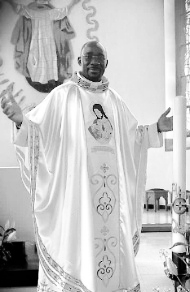
\includegraphics[scale=1.20]{../images/standing_daniel}
\end{wrapfigure}
Cette année nous porterons ensemble cette rentrée dans le cœur de chacun avec nos \textbf{jeunes pro}. Chacun à son rythme, selon ses possibilités et ses réalités mais avec un seul et même objectif : l’accomplissement de nos activités communautaires. Présentons également notre rentrée paroissiale au Christ. Et continuons notre chemin pour la mise en œuvre de notre projet paroissial autour de ce principal thème : \textbf{\og Avec notre jeunesse bâtissons une communauté plus dynamique, rayonnante et missionnaire\fg{}.}

	Que cette rentrée pastorale nous aide à prendre des résolutions nécessairement pour plonger à frais nouveaux dans la parole et être des disciples crédibles de l’évangile.


\begin{flushright}
Bonne rentrée pastorale à toutes et à tous !
\textit{Père  Daniel  ETTÉ}
\end{flushright}


\end{minipage}
%\end{center}
% -----
\end{document} 
